%% LyX 2.3.6.1 created this file.  For more info, see http://www.lyx.org/.
%% Do not edit unless you really know what you are doing.
\documentclass[english]{article}
\usepackage[T1]{fontenc}
\usepackage[latin9]{inputenc}
\usepackage{textcomp}
\usepackage{amsmath}
\usepackage{graphicx}

\makeatletter
%%%%%%%%%%%%%%%%%%%%%%%%%%%%%% Textclass specific LaTeX commands.
\newenvironment{lyxlist}[1]
	{\begin{list}{}
		{\settowidth{\labelwidth}{#1}
		 \setlength{\leftmargin}{\labelwidth}
		 \addtolength{\leftmargin}{\labelsep}
		 \renewcommand{\makelabel}[1]{##1\hfil}}}
	{\end{list}}

\makeatother

\usepackage{babel}
\begin{document}
\title{Algorithmic Robotics And Motion Planning Project}

\maketitle
Barak Ugav 318336229

\subsubsection*{The Question}

We are given a point robot $P$ which is known to be in the interior
of some polygonal room $Q$ with $n$ vertices. The robot is equipped
with a depth sensor which evaluates the distance to the visible obstacle
in the pointed direction. Describe a data structure that can be constructed
during preprocessing of the room and can be used to efficiently calculate
all the points the robot might think he is after a single depth measurement
from an unknown position and rotation.

\subsubsection*{Motivation}

Such scenario can be applicable in real world cases, for example:
a rover lands on Mars, a map of whose terrain is available to it.
It looks about its position, and then infers its exact position on
the Martian surface. Another application comes from robots that follow
a planned path through a scene: the control systems that guide such
a robot along the planned path gradually accumulate errors due to
mechanical drift. Thus it is desirable to use localization from time
to time to verify the actual position of the robot in the map, and
apply corrections as necessary to return it to the planned path.

\newpage{}

\section*{Solution}

To answer a query of the described type, we will perform preprocessing
of the room, and calculate for each edge the ``visible'' region
from it, and when given a query of measurement $d$ we will search
all the edges that have a region at distance $d$ from it. For each
edge $e$, we will set it's 2D coordination system with its origin
at the first vertex of the edge when traversing on the room's borders
clockwise, the $x$ axis along the edge and the $y$ axis perpendicular
to the edge. For a fixed angle $\theta$, we would like to calculate
the distance to the nearest obstacle visible from the edge in angle
$\theta$ as a function of the distance $x$ from the edge origin.

Given a fixed angle $\theta$, fixed point $x_{0}$ along an edge
$e$, the line that goes through $(x_{0},0)$ with angle $\theta$
is $y=tan\theta(x-x_{0})$. Given an edge $e'$ with equation $y=mx+b$
relative to $e$ origins, the two lines intersection point is $\left(\frac{tan\theta x_{0}+b}{tan\theta-m},\frac{tan\theta(mx_{0}+b)}{tan\theta-m}\right)$,
and the distance to the intersection can be calculated as follows:

\[
\sqrt{\left(\frac{tan\theta(mx_{0}+b)}{tan\theta-m}\right)^{2}+\left(\frac{tan\theta x_{0}+b}{tan\theta-m}-x_{0}\right)^{2}}
\]

\[
=\sqrt{\frac{tan^{2}\theta(mx_{0}+b)^{2}+(mx_{0}+b)^{2}}{\left(tan\theta-m\right)^{2}}}=\sqrt{\frac{(mx_{0}+b)^{2}(tan^{2}\theta+1)}{\left(tan\theta-m\right)^{2}}}
\]

\[
=\sqrt{\frac{(mx_{0}+b)^{2}sec^{2}\theta}{\left(tan\theta-m\right)^{2}}}=\frac{(mx_{0}+b)sec\theta}{tan\theta-m}
\]

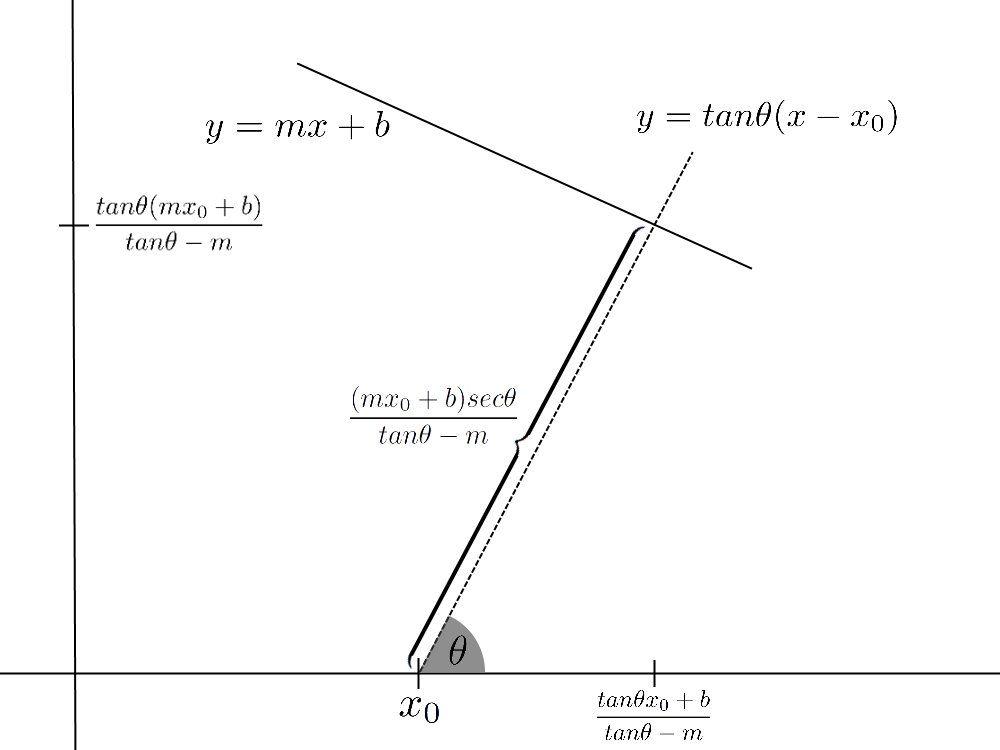
\includegraphics[scale=0.4,bb = 0 0 200 100, draft, type=eps]{figure4.png}

So we can write the visible distance of $e'$ from $e$ as a function
of $\theta,x_{0}$:

\[
f_{e,e'}(\theta,x)=\frac{(mx+b)sec\theta}{tan\theta-m}
\]

This is of course only defined if the intersection point is in $e'$
range and it's in the correct half plane of $e$. Note that $f_{e,e'}(\theta,x)$
is a straight line if $\theta$ is a fixed angle.

Denote $f_{e}(\theta,x)=\underset{e'}{min}\,f_{e,e'}(\theta,x)$.
For non fixed $\theta$, the function $f_{e}(\theta,x)$ represents
the maximum visible distance seen at $x$ on $e$ at angle $\theta$.

\subsection*{Discrete Angles Approach}

For our preprocessing, we will discretize the angle $\theta$, by
dividing it to $q$ (for example $1000$) small angles. For each fixed
angle $\theta$, will calculate for each edge $e$ the function $f_{e}(\theta,x)$.
For a fixed angle and edge, the visible edges can be changed at most
$O(n)$ times, because it can be changed only when a vertex is seen,
and no more than $n$ vertices can be seen, so $f_{e}(\theta,x)$
is composed from $O(n)$ intervals of $f_{e,e'}$ (of some $e'$).
There are two options in which we can define $\theta$:
\begin{lyxlist}{00.00.0000}
\item [{$\text{Relative angle:}$}] $\theta$ will be defined exactly as
described in the calculations above - the angle between the measurement
line and the measured edge. This can be used if somehow we know the
angle of our measurement and the measured edge. Will be used in ``Second
Measurement Variant - same edge''.
\item [{$\text{Absolute angle:}$}] $\theta$ will be defined as the angle
between the measurement line and the $x$ axis of the room. Note that
for a fixed $\theta$ defined like this, the \textbf{total} complexity
of all $\forall e,f_{e}(\theta,x)$ is $O(n)$, which is a stronger
claim than the above one on a single function $f_{e}(\theta,x)$.
\end{lyxlist}
We will alternate between these two approaches in different variants.
In the current setting, we will prefer to use an \textbf{absolute}
angle, this way the total complexity of all $f_{e}$ for a fixed angle
is $O(n)$. For each absolute angle $\theta$ we can calculate all
intervals of all edges in $O(nlogn)$ time by a plane sweep. Therefore
the preprocessing of all angles requires $O(qnlogn)$ time and $O(qn)$
space.

Given a query with distance $d$, we check for each edge $e$, and
each discretized angle $\theta$, all the intervals at which $f_{e}$
is greater than $d$, which we can calculate in time proportional
to the number of intervals. The result for the query is a set of all
the intervals of all angles and all edges that match the query. Therefore
the total time complexity for a query is $O(qn)$.

\newpage{}

\subsubsection*{Output Sensitive Optimizations}

The function $f_{e}(\theta,x)$ is composed of straight lines, denote
the $x$ intervals of these lines by $I_{i}^{e}$. Denote $max_{\theta}(I_{i}^{e})=\underset{x\in I_{i}^{e}}{max}\,f_{e}(\theta,x)$.
For a fixed edge $e$, we know if $d>max_{\theta}(I_{i}^{e})$, there
is no points in the room that the robot can be in to measure $d$
at $e$ at the $x$ interval $I_{i}^{e}$. We can use this to get
a more sensitive output algorithm. After the above preprocessing,
for each fixed angle $\theta$ and a fixed edge $e$ we calculate
for each interval the value $max_{\theta}(I_{i}^{e})$. We take the
total collection of all intervals of all angles and all edges sort
them by $max_{\theta}(I_{i}^{e})$. The preprocessing requires $O(qnlogqn)$
time and $O(qn)$ space.

Given a query with distance $d$, we only look at the angles and intervals
at which we know there will be a valid answer. Denote by $L$ the
number of different intervals of positions the robot can be relative
to any edge in any of the discrete angles. The time complexity of
the query is $O(logq+logn+L)$. In the worst case $L$ can be $O(qn)$.

In this setting, where we use discrete angles, and therefore the output
of any such algorithm will consist of a set of lines, $L$ is actually
proportional to the optimal solution length. We will assume from now
on a fixed angle $\theta$, as we compare our algorithm to an optimal
one which also outputs lines of fixed angles, and if their output
is proportional for a fixed angle, it is also proportional for all
the angles. Each interval of our algorithm must be included in the
optimal algorithm output, but the optimal algorithm may ``union''
some of our lines into one continuous one if possible to reduce the
output size. If a partial interval was outputted from our algorithm
(left figure), meaning part of the line the interval represents is
not valid, the optimal algorithm must also output only a part of it,
and we can ``associate'' our interval with the output algorithm
endpoint of the line (the endpoint which is included in our interval,
$c_{1}$). If a full interval was outputted from our algorithm (right
figure), we ``associate'' it with the endpoint of the line in the
opposite angle of the edge of the vertex that caused our interval
to terminate ($c_{2}$).

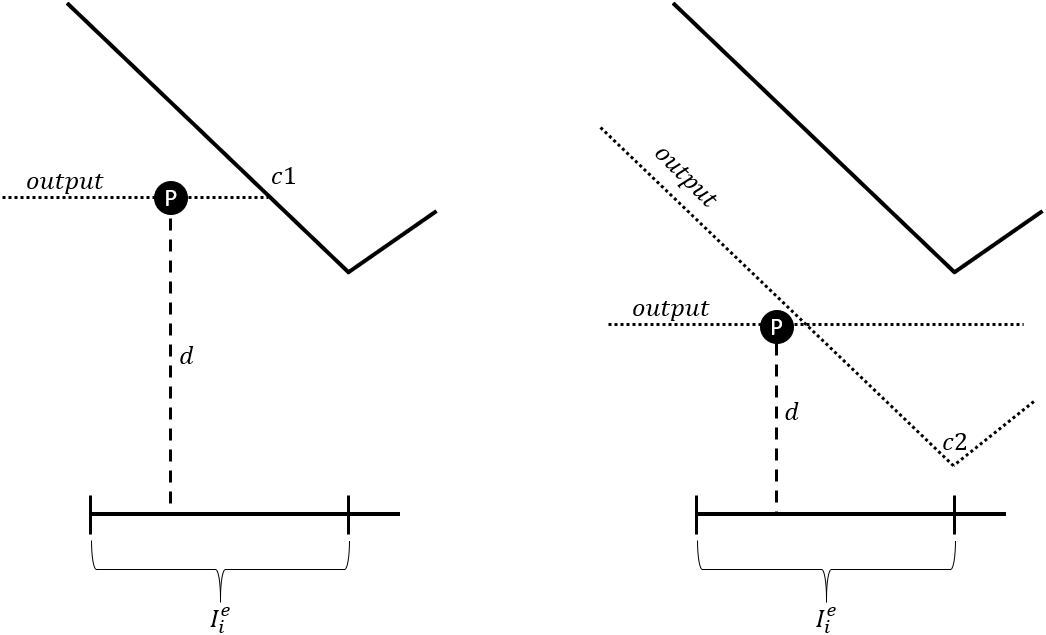
\includegraphics[scale=0.35,bb = 0 0 200 100, draft, type=eps]{figure6.png}

Therefore, for a fixed angle, we can associate each of our algorithm
output intervals to one of the optimal algorithm output vertices,
and no more than two intervals are associated with each vertex, and
if we look at all the angles together, $L$ is proportional to an
optimal output length.

\newpage{}

\subsubsection*{Second Measurement Variant - same edge }

If we are given the ability to measure a second distance measurement,
after the first measurement of $d_{1}$ we can turn the robot a small
angle $\epsilon$ without changing its position and measure a second
time a distance $d_{2}$. If we assume the turn we did is small enough,
we can assume we measured the same edge. Denote $\alpha=\epsilon$,
the difference along the edge between the two measurements by $c$
and $\theta$ the angle of the first measurement \textbf{relative}
to the edge. We can calculate $\theta$ as follows:

\[
c=\sqrt{d_{1}^{2}+d_{2}^{2}-2d_{1}d_{2}cos\alpha}
\]

\[
\theta=cos^{-1}\left(\frac{d_{1}^{2}+c^{2}-d_{2}^{2}}{2d_{1}c}\right)
\]

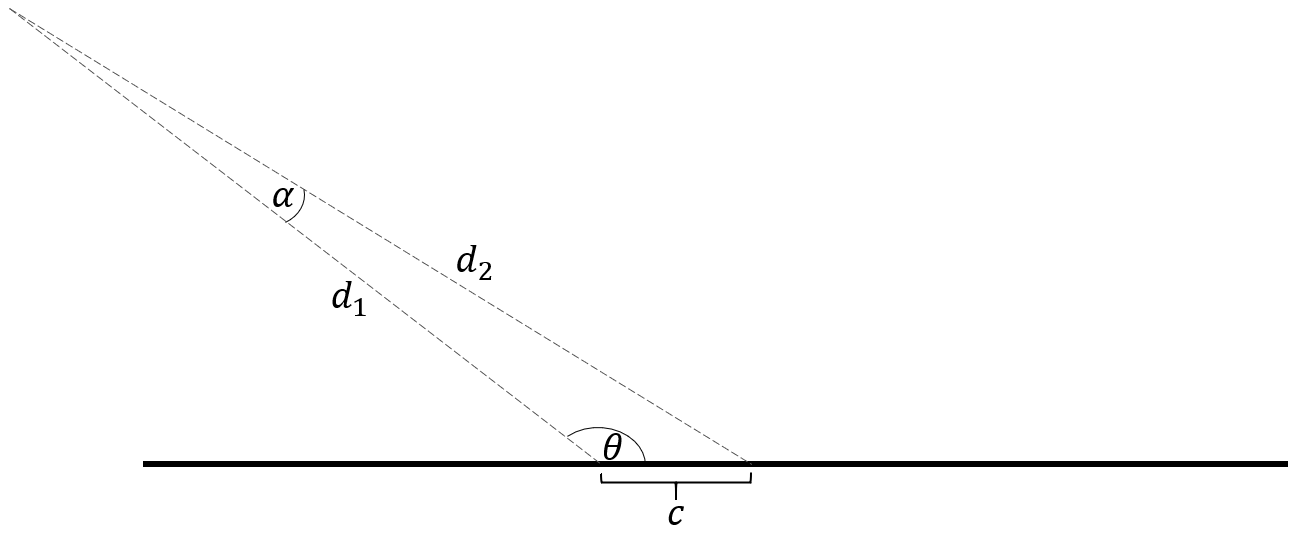
\includegraphics[scale=0.27,bb = 0 0 200 100, draft, type=eps]{figure5.png}

So given the angle between the measurement and the measured edge,
we can use the same data structure as before, but this time with \textbf{relative
}$\theta$, and instead of considering all the possible angles, consider
only the two angles which are most close to $\theta$ in our discrete
angles representation. This increases the preprocessing to $O(qn^{2}logqn)$
time and $O(qn^{2})$ space (as the total number of intervals per
$\theta$ can now be $O(n^{2})$) and reduces the query complexity
to $O(logn+L)$, but $L$ is expected to be much smaller but can be
$O(n^{2})$ in the worst case.

\subsubsection*{Second Measurement Variant - different edge }

After the robot performed a single measurement $d_{1}$, if we can't
assume we will always measure the same edge by turning a small angle,
we can guarantee a second measurement to a different edge by turning
$180\text{�}$, denoted $d_{2}$. Then we can use the definitions
as described above, and calculate another field for each interval
$min_{\theta}(I_{i}^{e})=\underset{x\in I_{i}^{e}}{min}\,f_{e}(\theta,x)$.
The robot could have measured $e$ at angle $\theta$ a distance $d_{1}$
and a second measurement $d_{2}$ only if $min_{\theta}(I_{i}^{e})\leq d_{1}+d_{2}\leq max_{\theta}(I_{i}^{e})$.
In preprocessing, we can build an interval tree (data structure of
number intervals) of the intervals $[min_{\theta}(I_{i}^{e}),max_{\theta}(I_{i}^{e})]$
which we can build in $O(qnlogqn)$ time. Given a query $(d_{1},d_{2})$
we search in the interval tree the value $d_{1}+d_{2}$ which takes
$O(logn+logq+L)$ where $L$ is the number of intervals that match
the query. For each interval we find in the interval tree we will
output a single point (or all the interval points, if the two edges
are parallel).
\end{document}
